\chapter{RESULTADOS}\label{chap:resultados}

Uma implementação do algoritmo EGSIS foi realizada como um projeto de
código-aberto e está disponível na plataforma
github\footnotemark. Nessa seção de resultados, avalia-se o
comportamento do método com variações no número de superpixels e
método de extração de características. Como referência para comparação
dos resultados, considera-se os métodos avaliados
em~\citeonline{wang2023review} no \textit{dataset} GrabCut.

\footnotetext{Disponível em \url{https://github.com/ryukinix/egsis/releases/tag/0.1.0}}

Uma avaliação qualitativa é demonstrada ao realizar a segmentação do
método e disponibilizar a máscara de segmentação gerada para algumas
imagens. Além disso, em formato de tabelas, é disponibilizada a
avaliação quantitativa baseada nas métricas descritas na
Seção~\ref{sec:metricas-avaliacao}.

Por fim, foi desenvolvida uma ferramenta simples de anotação para
exploração dos resultados integrada ao software
JupyterLab\footnotemark, que é usada também para avaliação qualitativa
e visualização do impacto da anotação parcial inicial no resultado
final.

\footnotetext{Software web para desenvolvimento interativo e análise de dados, disponível em \url{https://jupyter.org}}

\section{Experimentos com a variação da quantidade de superpixels}\label{sec:variacao-superpixels}

Durante a execução dos experimentos, e avaliação dos resultados, foi
observado que o número de superpixels afeta diretamente a qualidade da
segmentação gerada. Entre esses experimentos, foram realizadas 8
execuções com variações na técnica de extração de características
usada e no número de superpixels, sendo o número de superpixels
avaliados para 50, 100, 150 e 200.

\begin{table}[!h]
    \centering
    \Caption{\label{tab:variacao-superpixels} Resultados dos
experimentos ao variar o número de superpixels e o método de extração
de características. Em negrito os melhores resultados.}
  \begin{tabular}{lccccc}
    \toprule
    \textbf{Método}                  & \textbf{Recall} & \textbf{Precision} & \textbf{F1}     & \textbf{IoU}    & \textbf{Tempo (s)} \\
    \midrule \midrule
    $\gls{EGSIS}(s=50, f=gabor)$     & 0,7882          & 0,9225             & 0,8414          & 0,7412          & 9,22             \\
    $\gls{EGSIS}(s=100, f=gabor)$    & 0,8592          & 0,9505             & 0,8992          & 0,8232          & 14,78            \\
    $\gls{EGSIS}(s=150, f=gabor)$    & 0,8691          & 0,9550             & 0,9066          & 0,8354          & 18,44            \\
    $\gls{EGSIS}(s=200, f=gabor)$    & 0,8799          & \textbf{0,9620}    & 0,9167          & 0,8511          & 21,06            \\
    $\gls{EGSIS}(s=50, f=comatrix)$  & 0,7882          & 0,9225             & 0,8414          & 0,7412          & \textbf{4,94}    \\
    $\gls{EGSIS}(s=100, f=comatrix)$ & 0,8617          & 0,9510             & 0,9010          & 0,8259          & 11,26            \\
    $\gls{EGSIS}(s=150, f=comatrix)$ & 0,8777          & 0,9552             & 0,9125          & 0,8441          & 15,12            \\
    $\gls{EGSIS}(s=200, f=comatrix)$ & \textbf{0,8877} & 0,9611             & \textbf{0,9212} & \textbf{0,8578} & 19,08            \\
    \bottomrule
  \end{tabular}
  \Fonte{\fonteautor}
\end{table}

Ao analisar a Tabela~\ref{tab:variacao-superpixels}, é possível
perceber que o aumento de superpixels impacta positivamente na
qualidade da segmentação independente do método de extração de
características. A respeito do método de extração de características,
os resultados de ambos os métodos são próximos. Por outro lado, com
exceção da métrica de precisão, os melhores resultados vieram do
modelo com 200 superpixels e extração de características via matriz de
co-ocorrências. O aumento de superpixels também contribuí para o
aumento no tempo de execução do modelo. Não foi possível observar
melhora significativa nas métricas de avaliação ao usar mais de 200
superpixels, também notável observar que a melhora mais significativa
ocorre ao aumentar de 50 para 100 superpixels. Para poucos
superpixels, o tempo de execução é significativamente menor ao usar
matriz de co-ocorrências invés de filtros de gabor.

Todos os experimentos deste trabalho foram executados em um notebook
pessoal modelo \textit{Thinkpad E480}, com processador \textit{Intel i5{-}8250U @
3.400GHz}, 16GB de memória \textit{RAM} e sistema operacional \textit{Ubuntu 22.04.3
LTS}.


\section{Avaliação qualitativa}

Nesta avaliação qualitativa, é comparada visualmente a qualidade
de segmentação do método \gls{EGSIS} com os melhores parâmetros
encontrados na seção anterior, isto é, número de superpixels definido
para 200 e método de extração de características via matriz de
co-ocorrências.

Como referência, o artigo~\cite{wang2023review} contém execuções
comparativas de vários métodos na base de dados GrabCut. Neste artigo,
é selecionada uma comparação com 16 imagens, nas quais 7 diferentes
métodos de segmentação interativa foram usados.

\begin{figure}[h!]
        \captionsetup{width=16cm}
		\Caption{\label{fig:grabcut-comparacao}
          Comparação entre diferentes métodos de segmentação interativa no dataset GrabCut.
        }
		\centering
		\UFCfig{}{\fbox{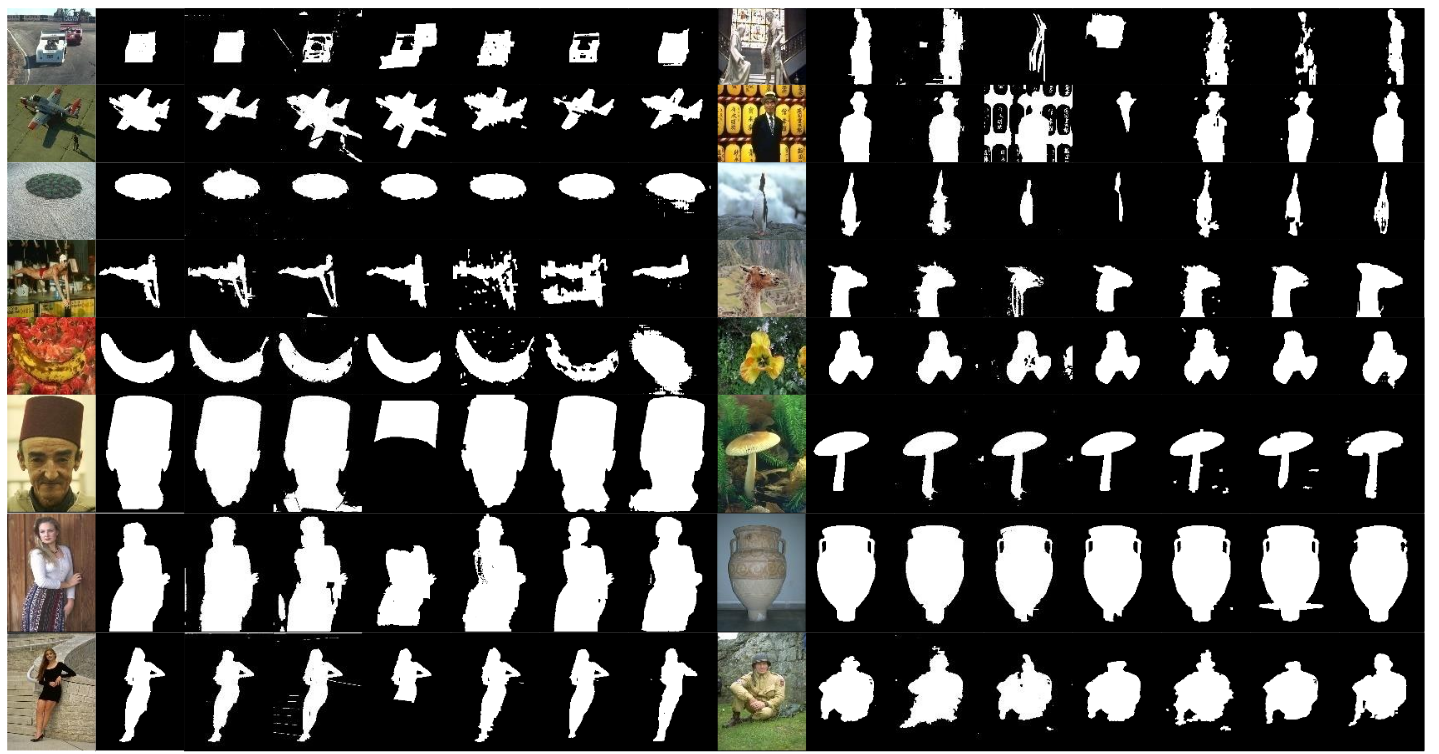
\includegraphics[width=16cm]{figuras/grabcut-comparacao}}}{\Fonte{\citeonline{wang2023review}}}
\end{figure}
\FloatBarrier{}

Na Figura~\ref{fig:grabcut-comparacao}, há em cada linha duas
imagens a serem segmentadas. Entre as máscaras de segmentação em escala
de cinza, há as segmentações dos métodos de segmentação
interativa. O nome desses 7 métodos, em ordem, são: GrabCut,
LazySnapping, OneCut, Saliency Cut, Iterated Graph Cuts\footnotemark{}, DenseCut e
Deep GrabCut.


\footnotetext{Não há um nome formal pra esse método~\cite{an2013iterated}, por ora ele será chamado assim.}

Nesse aspecto, para comparação com o modelo proposto \gls{EGSIS}, para
as mesmas imagens do dataset GrabCut, são obtidas as seguintes máscaras
de segmentação na Figura~\ref{fig:egsis-qualitativa}.

\begin{figure}[h!]
        \captionsetup{width=11.5cm}
		\Caption{\label{fig:egsis-qualitativa}
          Execuções de várias segmentações interativas com EGSIS.\@ A coluna ao
lado da imagem mostra a segmentação binária feita pelo modelo, e a
próxima coluna mostra a segmentação real.
        }
		\centering
		\UFCfig{}{\fbox{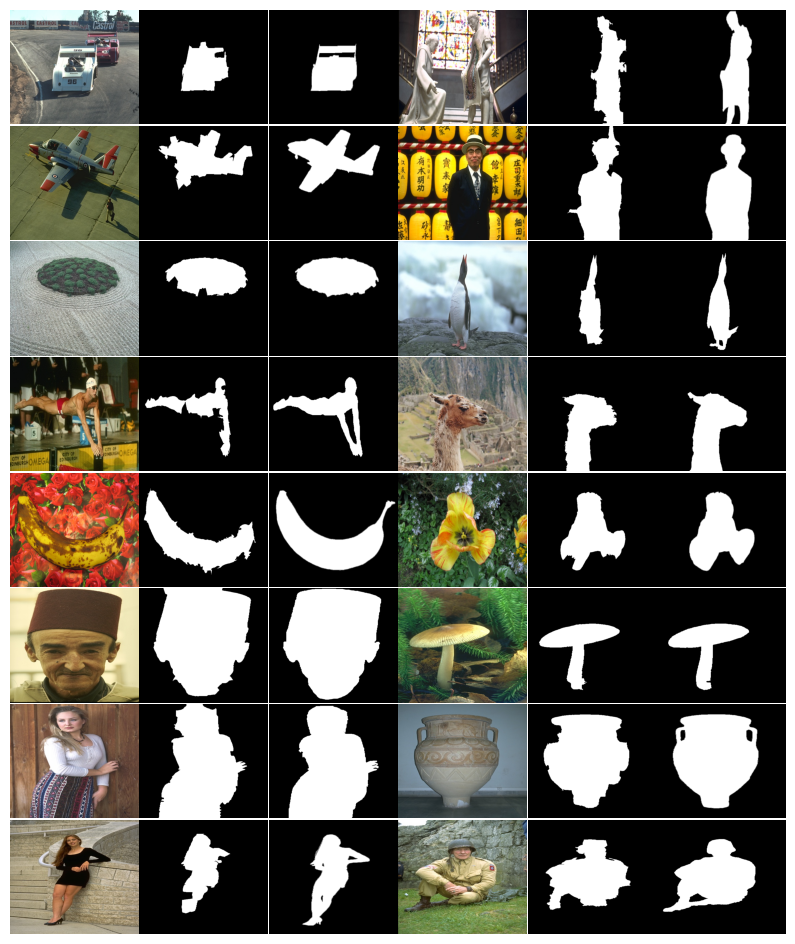
\includegraphics[width=11.5cm]{figuras/egsis-qualitativa}}}{\Fonte{\fonteautor}}
\end{figure}
\FloatBarrier{}



Como pode ser visto, os resultados do \gls{EGSIS} são de qualidade
equiparável aos métodos de referência em~\citeonline{wang2023review}, embora em
algumas imagens haja mais erros e outras obtenham maior êxito. Para
quantificar esse resultado, na próxima Seção~\ref{sec:comparacao-estado-da-arte} é realizada uma avaliação
quantitativa comparando esses métodos e o método proposto \gls{EGSIS}.


\section{Comparação quantitativa com o estado-da-arte da segmentação interativa}\label{sec:comparacao-estado-da-arte}

Nesta seção, é proposta uma avaliação de como o modelo \gls{EGSIS} se
compara ao estado-da-arte no problema de segmentação interativa.

No artigo de~\citeonline{wang2023review}, é observado um extenso estudo de
revisão sobre os métodos de segmentação interativa baseados em grafos,
tendo como base o algoritmo GrabCut e outros algoritmos que evoluíram
nessa área de segmentação interativa de imagens. Os autores avaliam
essas técnicas na base de dados GrabCut~\cite{rother2004grabcut}
utilizando as mesmas métricas que foram selecionadas na metodologia de
avaliação deste trabalho, com exceção do tempo de execução, que, por
conta de diferentes tecnologias usadas para implementação das
técnicas, não foi possível usar para fazer uma avaliação justa, por
isso será deixada como um potencial trabalho futuro.

Esse mesmo artigo também avalia as várias técnicas em outro
\textit{dataset}, mas em virtude de a rotulação inicial usada não ter
sido publicada, não foi possível replicar os experimentos para o
modelo \gls{EGSIS} nas mesmas condições. Por esse motivo, a avaliação
de resultados será limitada a base de dados GrabCut.

A seguir, é possível visualizar tabelas de comparação com os
algoritmos apresentados em~\citeonline{wang2023review}, todos
algoritmos de segmentação interativa baseado em grafos.


\begin{table}[!h]
  \centering
  \Caption{\label{tab:resultados-estado-da-arte} Resultados
    comparativos entre o método EGSIS e métodos estado-da-arte para
    segmentação interativa baseado em grafos. Em negrito os melhores
    resultados, em vermelho os piores.}
  \begin{tabular}{lcccc}
    \toprule
    \textbf{Método}                  & \textbf{Recall} & \textbf{Precision} & \textbf{F1}     & \textbf{IoU}    \\
    \midrule \midrule
    GrabCut                          & 0,9668          & 0,9213             & \textbf{0,9407} & \textbf{0,8927} \\
    LazySnapping                     & \textbf{0,9681} & 0,9104             & 0,9357          & 0,8842          \\
    OneCut                           & 0,8585          & \red{0,7926}       & \red{0,7899}    & \red{0,6974}    \\
    Saliency Cuts                    & \red{0,8371}    & 0,8892             & 0,8255          & 0,7458          \\
    Iterated Graph Cuts              & 0,9614          & 0,8878             & 0,9212          & 0,8597          \\
    DenseCut                         & 0,8427          & 0,9418             & 0,8561          & 0,7927          \\
    Deep GrabCut                     & 0,8854          & 0,8774             & 0,8701          & 0,7849          \\
    $\gls{EGSIS}(s=200, f=gabor)$    & 0,8799          & \textbf{0,9620}    & 0,9167          & 0,8511          \\
    $\gls{EGSIS}(s=200, f=comatrix)$ & 0,8877          & 0,9611             & 0,9212          & 0,8578          \\
    \bottomrule
  \end{tabular}
  \Fonte{Baseado nos resultados encontrados no artigo de~\citeonline{wang2023review}}
\end{table}
\FloatBarrier{}

\begin{table}[!h]
  \centering
  \Caption{\label{tab:resultados-egsis-desvio-padrao} Resultados do modelo EGSIS com desvio padrão.}
  \begin{tabular}{lcc}
    \toprule
    \textbf{Métrica}   & $\gls{EGSIS}(s=200, f=gabor)$ & $\gls{EGSIS}(s=200, f=comatrix)$ \\
    \midrule \midrule
    \textbf{Recall}    & 0,8799 $\pm$ 0,0907             & 0,8877 $\pm$ 0,0773                \\
    \textbf{Precision} & 0,9620 $\pm$ 0,0314             & 0,9611 $\pm$ 0,0347                \\
    \textbf{F1}        & 0,9167 $\pm$ 0,0581             & 0,9212 $\pm$ 0,0506                \\
    \textbf{IoU}       & 0,8511 $\pm$ 0,0942             & 0,8578 $\pm$ 0,0838                \\
    \bottomrule
  \end{tabular}
  \Fonte{Elaborado pelo autor.}
\end{table}
\FloatBarrier{}


Na Tabela~\ref{tab:resultados-estado-da-arte}, é possível
observar que o método $\gls{EGSIS}(s=200, f=gabor)$ atinge o maior
valor médio de precisão entre todos os métodos comparados, com um
valor de 0,9620. Seguindo o método EGSIS, o segundo colocado na
métrica de precisão foi o método DenseCut, com um valor de precisão de
0,9418, que é próximo, mas ainda significativamente menor. É
importante ressaltar que uma alta precisão implica uma baixa
incidência de pixels falsos-positivos.

Na Tabela~\ref{tab:resultados-egsis-desvio-padrao}, é possível
visualizar os resultados da média e do desvio padrão de cada métrica
de avaliação. Ao fazer uma análise incluindo o desvio padrão, não se
pode concluir estatisticamente qual melhor método de extração de
características, seja a matriz de co-ocorrências ou os filtros de
Gabor. Em todas as métricas há uma intersecção dos valores médios
quando se considera o desvio padrão.

Em nenhuma das métricas apresentadas na comparação o EGSIS se
classifica como o pior método. No entanto, observa-se um valor menor
de \textit{recall} em comparação à precisão, o que impacta diretamente
no valor das métricas \textit{F1} e IoU. Neste cenário, conclui-se que
o modelo EGSIS tem uma taxa maior de falsos-negativos do que de
falsos-positivos.

Embora seja necessária uma investigação mais aprofundada para
determinar a causa dessa maior taxa de falsos-negativos, é importante
notar que o conjunto de dados GrabCut possui um desequilíbrio na
quantidade de pixels entre as classes, sendo o plano de fundo a classe
dominante. No algoritmo \gls{LCU}, um dos fatores importantes para
classificar um vértice que representa um superpixel é a extração de
características que através de uma função de similaridade calcula o
peso das arestas da rede complexa. No entanto, esse é apenas um dos
fatores do sistema dinâmico, pois também há a geração de partículas e
a transição entre os vértices. Geralmente, o objeto é cercado pelo
plano de fundo. Isso pode levar a uma situação onde a rede complexa
maior, localizada fora do objeto, gera partículas da classe do plano
de fundo em quantidade suficiente para dominar os vértices na região
do objeto. Esse comportamento implicaria um aumento na incidência de
falsos-negativos.

Se isso for confirmado, uma possível contramedida seria modificar o
sistema dinâmico para dar maior peso às similaridades entre
superpixels, de tal maneira que haja um aumento da probabilidade
de sobrevivência das partículas entre superpixels de mesma
classe. Além disso, seria útil explorar novas técnicas de extração de
características que gerem valores de similaridade mais
discriminantes.

\section{Ferramenta de anotação integrada com método EGSIS}\label{sec:ferramenta-anotacao}

Para a exploração e avaliação dos resultados a nível individual de
imagem, desenvolveu-se uma ferramenta de anotação parcial de imagens
para testar o método EGSIS.\@ Esta ferramenta é utilizada no cenário de
segmentação interativa e seu uso é descrito nesta seção.


\begin{figure}[h!]
        \captionsetup{width=16cm}
		\Caption{\label{fig:annotator-label-annotation}
          Ferramenta para anotação parcial de imagem, com pontos
circulares e classes distintas por cor.
        }
		\centering
		\UFCfig{}{\fbox{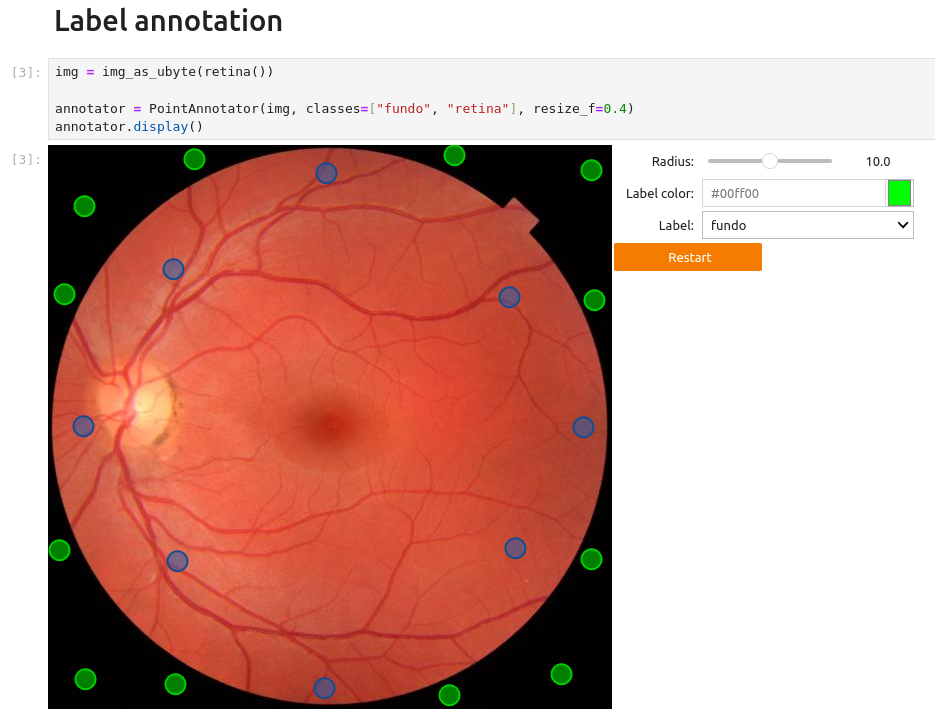
\includegraphics[width=16cm]{figuras/annotator-label-annotation}}}{\Fonte{\fonteautorscikit}}
\end{figure}
\FloatBarrier{}


A Figura~\ref{fig:annotator-label-annotation} ilustra a ferramenta
desenvolvida. Durante a inicialização do anotador, é possível declarar
o nome das classes a serem anotadas e selecionar a cor das anotações
{---} neste caso, verde para o plano de fundo e azul para a retina. A
cada clique do mouse, um ponto circular com raio variável pode ser
anotado, cujo tamanho pode ser definido pela ferramenta através de um
botão deslizante. Por fim, obtém-se uma instância do anotador que
contém as anotações e que pode ser usada para gerar uma matriz de
rótulos por pixel.

\begin{figure}[h!]
        \captionsetup{width=16cm}
		\Caption{\label{fig:annotator-egsis-execution}
          Execução do método EGSIS com a matriz de rótulos gerada pelo anotador.
        }
		\centering
		\UFCfig{}{\fbox{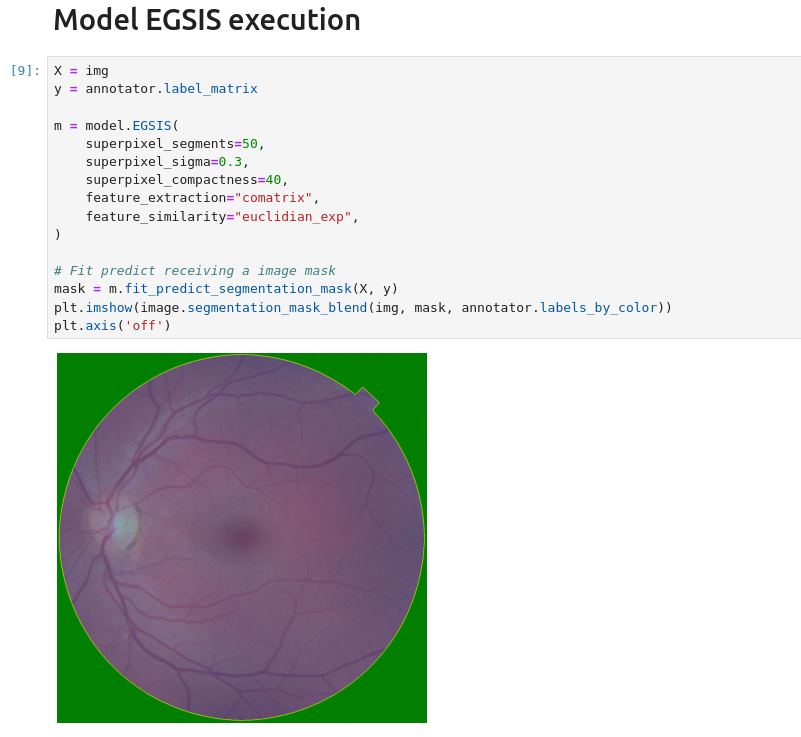
\includegraphics[width=16cm]{figuras/annotator-egsis-execution}}}{\Fonte{\fonteautorscikit}}
\end{figure}
\FloatBarrier{}

Na Figura~\ref{fig:annotator-egsis-execution}, a execução do algoritmo
EGSIS é ilustrada utilizando os dados de anotação como matriz de
rótulos $y$, que contém as anotações parciais. Ao final da execução, a
máscara de segmentação colorida é exibida sobreposta à imagem
original. Nessa situação, uma segmentação perfeita foi alcançada após
corrigir os erros do modelo na ferramenta de anotação com novos
pontos.
